\documentclass[serif]{beamer}\usepackage[]{graphicx}\usepackage[]{color}
%% maxwidth is the original width if it is less than linewidth
%% otherwise use linewidth (to make sure the graphics do not exceed the margin)
\makeatletter
\def\maxwidth{ %
  \ifdim\Gin@nat@width>\linewidth
    \linewidth
  \else
    \Gin@nat@width
  \fi
}
\makeatother

\definecolor{fgcolor}{rgb}{0.345, 0.345, 0.345}
\newcommand{\hlnum}[1]{\textcolor[rgb]{0.686,0.059,0.569}{#1}}%
\newcommand{\hlstr}[1]{\textcolor[rgb]{0.192,0.494,0.8}{#1}}%
\newcommand{\hlcom}[1]{\textcolor[rgb]{0.678,0.584,0.686}{\textit{#1}}}%
\newcommand{\hlopt}[1]{\textcolor[rgb]{0,0,0}{#1}}%
\newcommand{\hlstd}[1]{\textcolor[rgb]{0.345,0.345,0.345}{#1}}%
\newcommand{\hlkwa}[1]{\textcolor[rgb]{0.161,0.373,0.58}{\textbf{#1}}}%
\newcommand{\hlkwb}[1]{\textcolor[rgb]{0.69,0.353,0.396}{#1}}%
\newcommand{\hlkwc}[1]{\textcolor[rgb]{0.333,0.667,0.333}{#1}}%
\newcommand{\hlkwd}[1]{\textcolor[rgb]{0.737,0.353,0.396}{\textbf{#1}}}%

\usepackage{framed}
\makeatletter
\newenvironment{kframe}{%
 \def\at@end@of@kframe{}%
 \ifinner\ifhmode%
  \def\at@end@of@kframe{\end{minipage}}%
  \begin{minipage}{\columnwidth}%
 \fi\fi%
 \def\FrameCommand##1{\hskip\@totalleftmargin \hskip-\fboxsep
 \colorbox{shadecolor}{##1}\hskip-\fboxsep
     % There is no \\@totalrightmargin, so:
     \hskip-\linewidth \hskip-\@totalleftmargin \hskip\columnwidth}%
 \MakeFramed {\advance\hsize-\width
   \@totalleftmargin\z@ \linewidth\hsize
   \@setminipage}}%
 {\par\unskip\endMakeFramed%
 \at@end@of@kframe}
\makeatother

\definecolor{shadecolor}{rgb}{.97, .97, .97}
\definecolor{messagecolor}{rgb}{0, 0, 0}
\definecolor{warningcolor}{rgb}{1, 0, 1}
\definecolor{errorcolor}{rgb}{1, 0, 0}
\newenvironment{knitrout}{}{} % an empty environment to be redefined in TeX

\usepackage{alltt}
\usetheme{Boadilla}
\usetheme{Boadilla}
\usepackage{graphicx}
\usepackage[final]{animate}
\usepackage{breqn}
\usepackage{xcolor}
\usepackage{booktabs}
\usepackage{tikz}
\usetikzlibrary{decorations.pathreplacing}
\usetikzlibrary{shapes,arrows,positioning,shadows}
\definecolor{links}{HTML}{2A1B81}
\hypersetup{colorlinks,linkcolor=links,urlcolor=links}
\usepackage{subfig}
\usepackage{pgf}
\usepackage{pgffor}

% knitr and global options


% load R libraries


\newcommand{\Bigtxt}[1]{\textbf{\textit{#1}}}
\IfFileExists{upquote.sty}{\usepackage{upquote}}{}
\begin{document}

\title[Comparison of WRTDS and GAMs]{Comparison of WRTDS and GAMs for evaluting long-term trends in chlorophyll}

\author[Beck, Murphy]{Marcus W. Beck\inst{1} \and Rebecca Murphy\inst{2}}

\date{April 30, 2015}

\institute[]{\inst{1} ORISE post-doc, USEPA National Health and Environmental Effects Research Laboratory, Gulf Ecology Division, \href{mailto:beck.marcus@epa.gov}{beck.marcus@epa.gov} \and \inst{2} Chesapeake Bay Program, \href{mailto:rmurphy@umces.edu}{rmurphy@umces.edu}}

%%%%%%
\begin{frame}
\titlepage
\end{frame}

%%%%%%
\begin{frame}{Today's call}
\begin{itemize}
\item Motivation for the analysis \\~\\
\item Site selection \\~\\
\item Exploratory evaluation of trends \\~\\
\item Initial applications of WRTDS/GAMS \\~\\
\item Group discussion (and throughout) 
\end{itemize}
\end{frame}

%%%%%%
\begin{frame}{Study motivation}
\begin{itemize}
\item WRTDS and GAMS recently used to evaluate water quality trends in tidal waters \\~\\
\item The relative values of each approach have not been evaluated - empirical description, desired products \\~\\
\item Comparisons could inform use of each model for management/restoration or for describing long-term changes \\~\\
\end{itemize}
\Bigtxt{Goal: Provide a description of the relative abilities of GAMs and WRTDS to describe long-term changes in time series of response endpoints in tidal waters}
\end{frame}

%%%%%%
\begin{frame}{Objectives}
\begin{itemize}
\item Provide a narrative comparison of the statistical foundation, both as a general description and as a means to evaluate water quality trends \\~\\
\item Use each technique to describe water quality changes in a common dataset with known historical changes in water quality drivers \\~\\
\item Compare each technique's ability to describe changes, as well as the differences in the information provided by each \\~\\
\item Apply to simulated data to evaluate the ability to reproduce flow-normalized trends
\end{itemize}
\end{frame}

%%%%%%
\begin{frame}{Site selection}
\begin{columns}[T]
\begin{column}{0.45\textwidth}
Monitoring stations in the Patuxent River Estuary... \\~\\
\begin{itemize}
\item longitudinal gradient from watershed to mainstem influences \\~\\
\item hurricane impacts \\~\\
\item well-studied (Testa, Kemp, Hagy, etc.)
\end{itemize}
\end{column}
\begin{column}{0.45\textwidth}
\centerline{\fbox{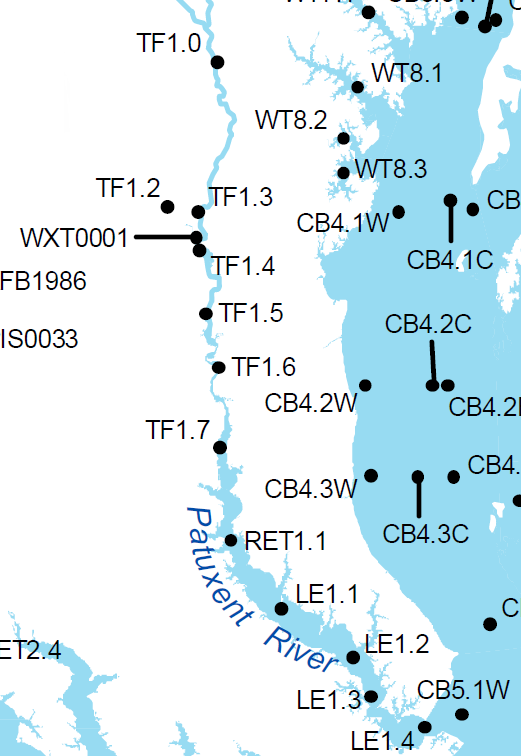
\includegraphics[width = 0.9\textwidth]{M:/docs/tidal_comp/figs/stations.png}}}
\end{column}
\end{columns}
\end{frame}

%%%%%%
\begin{frame}{Site selection}
\begin{columns}[T]
\begin{column}{0.45\textwidth}
Monitoring stations in the Patuxent River Estuary... \\~\\
\begin{itemize}
\item TF1.7, LE1.1 based on data distribution - monthly from 1986 -- 2014\\~\\
\item surface chlorophyll only (okay?)  \\~\\
\item vertically integrated salinity \\~\\
\item No detection limit issues
\end{itemize}
\end{column}
\begin{column}{0.45\textwidth}
\centerline{\fbox{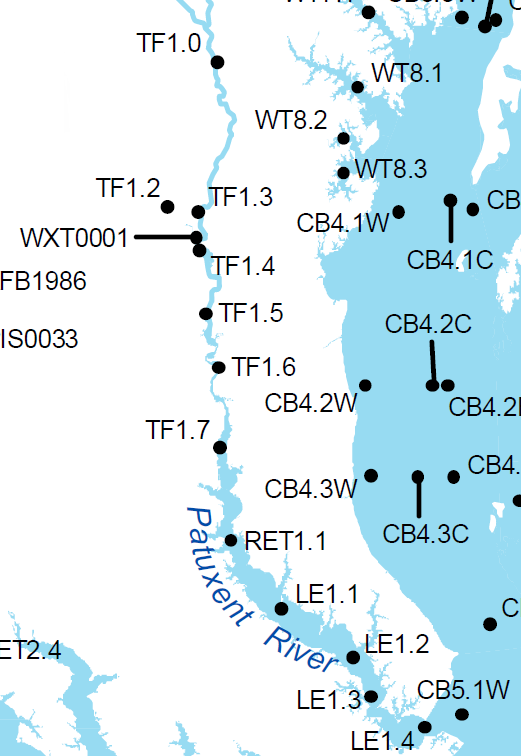
\includegraphics[width = 0.9\textwidth]{M:/docs/tidal_comp/figs/stations.png}}}
\end{column}
\end{columns}
\end{frame}

%%%%%%

\begin{frame}{Some exploratory graphs}
Summaries of annual and seasonal trends by station \\~\\
\begin{center}
\foreach \n in {1,...,10}{\includegraphics<\n>[width = \textwidth, page = \n]{figs/pax_chl.pdf}}
\end{center}
\end{frame}

%%%%%%

\begin{frame}{Some exploratory graphs}
Chlorophyll changes by month, annual aggregations \\~\\
\begin{center}
\foreach \n in {1,...,12}{\includegraphics<\n>[width = \textwidth, page = \n]{figs/pax_trnds.pdf}}
\end{center}
\end{frame}

%%%%%%

\begin{frame}{Some exploratory graphs}
Chlorophyll changes by year, monthly aggregations \\~\\
\begin{center}
\foreach \n in {1,...,29}{\includegraphics<\n>[width = \textwidth, page = \n]{figs/pax_yrtrnds.pdf}}
\end{center}
\end{frame}

%%%%%%
\begin{frame}{Initial application of WRTDS/GAMs}

\end{frame}

\end{document}
